\documentclass[parskip=full]{scrartcl}
\usepackage[utf8]{inputenc} % use utf8 file encoding for TeX sources
\usepackage[T1]{fontenc}    % avoid garbled Unicode text in pdf
\usepackage[german]{babel}  % german hyphenation, quotes, etc
\usepackage{hyperref}       % detailed hyperlink/pdf configuration
\usepackage{graphicx}       % provides commands for including figures
\usepackage{csquotes}       % provides \enquote{} macro for "quotes"
\usepackage[nonumberlist]{glossaries}     % provides glossary commands
\usepackage{enumitem}
\usepackage{setspace}
\usepackage{subfigure}
\usepackage{pgf}

\makenoidxglossaries

\newglossaryentry{nn}
{
	name={neural network},
	description={a network or a circuit of neuron used for information processing inspired by the way biological neural systems process data},
	plural=neural networks
}

\newglossaryentry{img}
{
	name={image},
	description={a two dimensional matrix of red,green,blue (RGB) values that can be visualized as each cell represents a single pixel on the monitor. (ex.: a photo)},
	plural=images
}

\newglossaryentry{cpu}
{
	name={CPU},
	description={Central Processing Unit},
	plural=CPUs
}

\newglossaryentry{fpga}
{
	name={FPGA},
	description={Field Programmable Gate Array},
	plural=FPGAs
}

\newglossaryentry{json}
{
	name={JSON},
	description={JavaScript Object Notation},
}

\newglossaryentry{xml}
{
	name={XML},
	description={Extensible Markup Language},
}

\title{Specifications}
\author{}
\begin{document}
\begin{titlepage}
\centering
	\vspace{3cm}
	{\scshape\LARGE Praxis der Softwarentwicklung\par}
	\vspace{2cm}
	{\scshape\Huge\bfseries Specificationsbook \par}	
	\vspace{2cm}
	{\scshape\Huge\bfseries Neural Network based Image Classification System on Heterogeneous Platforms \\ Team 2 \par}
	\vspace{2cm}
	{\Large from \par}
	\vspace{0.25cm}
	{\Large Häring, Stangel, Drehwald, Guneshka, Dimitrov \par}
	\vfill
\end{titlepage}
\newpage
\tableofcontents
\newpage
\section{Preface}

\section{Goal}
The goal is a software which performs image classification and is able to switch between deploy platforms and working modes.
It also should have a GUI to control the software and to show the results.

\section{Product use}
Image classification

\section{Acceptance criteria}
\subsection{Must}
\begin{tabular}{p{2cm}p{11.4cm}}
\textbf{AC10} & \textbf{Image classification} \\
& The software can take a single image as input and tell the user to which predifined class, if any, this image belongs.\\
\textbf{MAC020} & \textbf{Running \gls{nn} on a heterogeneous platform} \\
& The software is able to do the execution of a given neural network (inference) on different compute devices. At least one \gls{cpu} and one \gls{fpga} should be supported.
The user is able to choose which compute device should be used for his \gls{img}.\\
\textbf{AC30} & \textbf{Different operating modes} \\
& The software has three modes. One mode for high perfomance, one for low power consumption and one for high energy effiency. \\
\textbf{AC40} & \textbf{GUI for interacting with software} \\
& The user should be able to access the entire functionality described in AC10-AC50 just by using the functional GUI.\\ 
& No coding or command line usage is required.\\
\textbf{AC50} & \textbf{Performance and power consumption prediction}\\
& The software can predict the performance with a certain powerconsumption and also the powerconsumption for a certain performance.

\end{tabular}
%\begin{itemize}[nosep]
%\item [MAC010]: Image classification
%\item [MAC020]: Running NN on heterogenous platforms, CPU and FPGA
%\item [MAC030]: Different operating modes
%\item [MAC040]: GUI for interacting with software
%\item [MAC050]: Performance/power prediction
%\end{itemize}

\subsection{Can}
\begin{tabular}{p{2cm}p{11.4cm}}
\textbf{KAC070} & \textbf{Illustration of the topology of a nn} \\
& The software is able to visualize the topology of a given nn in a usefull way without requirering additional information. \\
& The visualized nn can be saved as a .png file\\
\textbf{KAC80} & \textbf{Object Detection} \\
&The software is able to not only say what kind of species there is on the picture, but also detect its outer points and draw a bounding box around it. \\ 
\textbf{KAC100} & \textbf{Creating new models} \\
& The software allows the user to train a neural network based on an architecture which the user developed.\\
& Neural networks created and trained by the user will be executed the same way neural networks provided with the software are executed.\\
\textbf{KAC110} & \textbf{Voting of multiple nn} \\
& The user is able to choose multiple nn for classification.\\
& The software will then execute all selected neural networks sequentially. The result presented to the User will be based on the weighted opinions of the different neural networks.\\
\textbf{KAC120} & \textbf{Using video for classification} \\
& The software is able to take a video, divide it in frames and perform image classification for each frame.\\
& The classified video can be viewed side by side as if changing to the next image at a constant rate and the classification could be saved as a \gls{json} or an \gls{xml} file.\\
\textbf{KAC130} & \textbf{Using camera for classification input} \\
& The software is able to take frames captured with a camera as an input and classify them.\\
& The process could take the current frame, classify it, display the results and then when ready, take the next available frame.
\end{tabular}
\begin{itemize}[nosep]
\item [KAC060]: Training a nn for classification
%\item [KAC070]: Illustration of the topology of a nn
%\item [KAC080]: Object detection
\item [KAC090]: Choosing between different models
%\item [KAC100]: Creating new models
%\item [KAC110]: Voting of multiple nn
%\item [KAC120]: Using video for classification
%\item [KAC130]: Using camera for classification input
\item [KAC140]: Running NN on GPU
\item [KAC150]: The GUI covers all implemented features in 4.1 and 4.2
\end{itemize}

\section{Functional Requirements Must}
\begin{itemize}[nosep]
\item [MFR025]: Dispatching the calculation process defined from the mode
\item [MFR030]: Support CPU for calculation
\item [MFR031]: Support FPGA for calculation
\item [MFR032]: Support GPU for calculation
\item [MFR040]: Communication between Host-PC and platform
\item [MFR041]: Send image for classification
\item [MFR042]: Receive result
\item [MFR050]: GUI
\item [MFR060]: Showing results
\end{itemize}
\begin{tabular}{p{2cm}p{11.4cm}}

\textbf{MFR010} & \textbf{Use \gls{nn} for \gls{img} classification}\\                                     
& A \gls{nn} should be used in order to classify \glspl{img} based on what is shown on them. For each \gls{img} a list of possible classes it could belong to along with degree of confidence should be given as output.\\
& \\
\textbf{MFR011} & \textbf{Deploy pre-trained \gls{nn} with the corresponding layers}\\
& A pre-trained \gls{nn} should be deployed to with all the corresponding layers in order to fulfill MFR010.\\
& \\
\textbf{MFR012} & \textbf{Reading and parsing \gls{nn} configuration/weight file}\\
& The software is able to a configuration file of a speciffic \gls{nn} and parse it for use in the classification.\\
& \\
\textbf{MFR020} & \textbf{Have high performance operating mode}\\                                     
& An option to perform calculations fast with low regard for power consumption.\\
\textbf{MFR021} & \textbf{Have low power consumption operating mode}\\                                     
& An option to perform calculations with low power consumption and low regard for speed.\\
& \\
\textbf{MFR022} & \textbf{Have high energy efficiency operating mode}\\                                     
& An option to perform calculations at an adequate balance between speed and power consumption.\\
& \\
\textbf{MFR023} & \textbf{Calculator for power consumption}\\                                     
& Calculations for the possible power consumption running the \gls{img} classifications would result in based on the \gls{nn}, platform and operating mode used.\\
& \\
\textbf{MFR024} & \textbf{Calculator for performance}\\                                     
& Calculations for the possible performance running the \gls{img} classifications would result in based on the \gls{nn}, platform and operating mode used.\\
& \\
\textbf{FR070} & \textbf{Choosing image for classification}\\
& Testet with: Implements: \\
& The GUI has a button with an on click event which opens a file explorer. The explorer filters the files so that only files of the format .jpg, .png, .bmp are listed. That also are the only valid formats.\\
\textbf{FR080} & \textbf{Choosing platform/hardware}\\
& Testet with: Implements: \\
& The GUI has a dropdown which lists the devices on which the classification can be done. The devices which can be theoretically be accessed but aren't connected to the host pc or the communication with them doesn't work are grayed out. \\
\textbf{FR090} & \textbf{Choosing mode}\\
& Testet with: Implements: \\
& The GUI has dropdown which lists the modes (high performance mode, low power consumption mode and best energy effiency mode). The power consumption in Watts and performance in FLOPs are also stated behind the mode names.
\end{tabular}

\section{Functional Requirements Can}
\begin{tabular}{p{2cm}p{11.4cm}}
\textbf{FR100} & \textbf{Choosing between different models}\\
& Testet with: Implements: \\
& The GUI has a button which opens the file explorer which filters for .txt files, there you choose the config file of the neural network with which you want to use. The program loads this config and parses it so it can be deployed. Possible models are GoogLeNet or AlexNet.\\
\textbf{FR110} & \textbf{Train nn for classification of imageset (with transfer learning)}\\
& Testet with: Implements: \\
& The user chooses a pretrained neural network and a new imageset and then can train the neural network on this new imageset with transfer learning.\\
%\newpage

\end{tabular}
\begin{itemize}[nosep]
%\item [KFR111]: Saving new trained nn (config an weights)
%\item [KFR112]: Choosing/Reading data set
\item [KFR032]: Support GPU for calculation
\item [KFR113]: Backpropagation
\item [KFR114]: Choosing parameters like learning rate
\item [KFR120]: Illustrating nn topology
\item [KFR130]: Object detection algorithm
\item [KFR131]: Showing detected object
\item [KFR132]: Choosing between detection and classification mode
%\item [KFR140]: Creating new topology
%\item [KFR150]: Choosing between training and interference mode
%\item [KFR160]: Choosing video in format .avi
%\item [KFR161]: Apply classification for a certain amount of frames
%\item [KFR170]: Connect with camera 
%\item [KFR171]: Receive video stream from camera
%\item [KFR180]: Detecting object
%\item [KFR181]: Drawing bounding box
\end{itemize}

\section{Productdata}
\begin{tabular}{p{2cm}p{11.4cm}}
\textbf{PD010} & \textbf{Images for classification}\\
& The user can choose images of the format .jpg, .png, .bmp. The images are chosen by the user with the file explorer.\\
\textbf{PD020} & \textbf{Config/weight file of pretrained model}\\
& It is a .cfg file. In the beginning are hyperparameters described with the format \textit{name = value}. Then the layers are described in their order with the following format\\
& \textit{\lbrack kind of layer\rbrack}\\
& list of parameters in the format \textit{name = value}\\
\textbf{PD030} & \textbf{Labeled image set for classification training}\\
& The dataset is chosen by the user. The dataset is a directory with images and the name of the image is the label.\\
\textbf{PD040} & \textbf{Labeled set of images for object detection training}\\
& It is a .txt file and a directory with images. The images are labeled with their name. The bounding box for each image are described in the .txt file, in the format \textit{imagename, x,y,width,height}. (X,Y) are the coordinates in pixel of the left bottom corner, the width and height are in pixel.
\end{tabular}

\section{Demarcation}
\begin{tabular}{p{2cm}p{11.4cm}}
\textbf{D010} & \textbf{No low-level optimization}\\
& Optimizations to reduce the execution time of object classification and detection will mainly be carried out in OpenCL.\\
& No optimizations including low-level languages or assembly intrinsics will be implemented.\\
&\\
\textbf{D020} & \textbf{No real time optimization}\\
& Common code optimizations will be done where possible to reduce the running time of the network per image classification/detection task.\\
& They do not have to lead to real-time reactions of the system.\\
& A computation time of multiple seconds per image is acceptable.\\
&\\
\textbf{D030} & \textbf{No neural network size optimization}\\
&No techniques for memory usage reduction like parameter sharing, prunning or binarization will be implemented.\\
&\\
\textbf{D040} & \textbf{No mobile support}\\
& There are no intentations to run any parts of this code on a mobile device like a smartphone or Augmented Reality glass.\\
& Mobile device requirements are not taken into consideration when choosing Techniques, languages and hardware used in this project. \\
&\\
\end{tabular}
%\begin{itemize}[nosep]
%\item [D020]: No real time / no performance optimization
%\item [D040]: No mobile support
%\item [D030]: No neural network size optimization
%\item [D010]: No low-level (Assembler) optimization
%\end{itemize}

\section{Non-functional requirements}
\begin{itemize}[nosep]
\item[NF10] 
\end{itemize}

\section{Test cases}
\begin{tabular}{p{2cm}p{11.4cm}}
\textbf{T010} & \textbf{Use \gls{nn} for \gls{img} classification}\\
& \textbf{State:} A \gls{img} is given as an input.\\
& \textbf{Action:} Calculations are performed on hand of the \gls{img} and a \gls{nn}.\\
& \textbf{Reaction:} A list of possible classes the given \gls{img} could belong to along with degree of confidence for each class are given as output.\\
& \\
\textbf{T011} & \textbf{Deploy pre-trained \gls{nn} with the corresponding layers}\\
& \textbf{State:} There is a \gls{nn} (already trained).\\
& \textbf{Action:} Calculations are performed cased on a given \gls{img} and the given \gls{nn}.\\
& \textbf{Reaction:} A list of possible classes the given \gls{img} could belong to along with degree of confidence for each class are given as output.\\
& \\
\textbf{T012} & \textbf{Reading and parsing \gls{nn} configuration/weight file}\\
T012.1 & \textbf{State:}  The user is on the page to select a \gls{nn} to use for the \gls{img} classification.\\
& \textbf{Action:} The user selects the option to import a \gls{nn}.\\
& \textbf{Reaction:} The file explorer opens.\\
T012.2 & \textbf{State:} The file explorer is open\\
& \textbf{Action:} The user selects an \gls{nn} to import\\
& \textbf{Reaction:} The file explorer closes and \gls{nn} is imported and selected for the classification calculations.\\
& \\
\textbf{T020} & \textbf{Have high performance operating mode}\\
& \textbf{State:} The user is ready to start the calculations.\\
& \textbf{Action:} The user chooses to perform the calculations in high performance operating mode.\\
& \textbf{Reaction:} The calculations run considerably faster than in the other possible modes with the same conditions.\\
& \\
\textbf{T021} & \textbf{Have low power consumption operating mode}\\
& \textbf{State:} The user is ready to start the calculations.\\
& \textbf{Action:} The user chooses to perform the calculations in low power consumption operating mode.\\
& \textbf{Reaction:} The calculations run with considerably lower power consumption than with the other possible modes in the same conditions.\\
& \\
\textbf{T022} & \textbf{Have high energy efficiency operating mode}\\
& \textbf{State:} The user is ready to start the calculations.\\
& \textbf{Action:} The user chooses to perform the calculations in high energy efficiency operating mode.\\
& \textbf{Reaction:} The calculations run with regard to balance between power consumption and speed.\\
& \\
%Manu quick fix:
\end{tabular}
\newpage
\begin{tabular}{p{2cm}p{11.4cm}}
\textbf{T040} & \textbf{Send image for classification} \\
T040.1 & \textbf{State:} The user in on the page for image classification \\
& \textbf{Action:} The user selects an image to be classificated.  \\
& \textbf{Reaction:} The software sends an array of pixels to the selected platform.\\
T040.2 & \textbf{State:} The software is awaiting result \\
& \textbf{Action:} Platform sends results \\
& \textbf{Reaction:} The software is expected to receive an array of changed pixels from the platform. \\ 
\textbf{T070} & \textbf{Choosing image for classification}\\
T070.1 & \textbf{State:} The user is on the page for image classification. \\
& \textbf{Action:} The user clicks on the button \glqq Choose image\grqq .\\
& \textbf{Reaction:} The file explorer opens with the filter for .png, .jpg, .bmp\\
T070.2 & \textbf{State:} The file explorer is open\\
& \textbf{Action:} The user selects an image with a valid format\\
& \textbf{Reaction:} The file explorer closes and image is as preview shown\\
\textbf{T080} & \textbf{Choosing platform/hardware}\\
T080.1 & \textbf{State:} The user is on the page for image classification\\
& \textbf{Action:} The user chooses with the dropdown the desired platform\\
& \textbf{Reaction:} An internal flag is set to the desired platform and the dropdown shows the chosen platform.\\
& \\
\textbf{T090} & \textbf{Choosing mode}\\
T090.1 & \textbf{State:} The user is on the page for image classification\\
& \textbf{Action:} The user chooses with the dropdown the desired mode\\
& \textbf{Reaction:} An internal flag is set to the desired mode and the dropdown shows the chosen mode\\
& \\
\textbf{T100} & \textbf{Choosing between different models}\\
T100.1 & \textbf{State:} The user is on the page for image classification\\
& \textbf{Action:} The user clicks on the button \glqq Choose neural network\grqq\\
& \textbf{Reaction:} The file explorer opens\\
T100.2 & \textbf{State:} The file explorer is open\\
& \textbf{Action:} The user selects an config/weight file\\
& \textbf{Reaction:} The file explorer closes and the software loads the input and parses it. If it is loaded there is success message\\
& \\
\textbf{T110} & \textbf{Train neural network for classification of imageset}\\
T110.1 & \textbf{State:} The user is on the page for training, has selected a neural network, a dataset for training, the kind of training, the learning rate and the desired precision.\\
& \textbf{Action:} The user clicks on the button \glqq Train\grqq\\
& \textbf{Reaction:} The software starts to train the selected network with the selected configuration and shows the progress in line graph.\\
& \\
%Manuel
\textbf{T111} & \textbf{Saving a NN after training}\\
T111.1 & \textbf{State:} The user is on the page for training, has selected a neural network, a dataset for training, the kind of training, the learning rate and the desired precision.\\
& The training finishes.\\
& \textbf{Action:} No action required\\
& \textbf{Reaction:} The software stores the trained network weights in a predifined format and with a usefull name in a fixed location.\\
& \\
%Manu quick fix:
\end{tabular}
\newpage
\begin{tabular}{p{2cm}p{11.4cm}}
\textbf{T112} & \textbf{Choosing/Reading data set}\\
T112.1 & \textbf{State:} A folder containing images is provided by the user.\\
& \textbf{Action:} No action required\\
& The software is able to read all images matching the allowed formats and allows training and inferencing on these images.\\

& \\
\textbf{T140} & \textbf{Creating new topology}\\
T140.1 & \textbf{State:} \\
& \textbf{Action:} No action required\\
& \textbf{Reaction:} \\
& A folder containing images is provided by the user.\\
& The software is able to read all images matching the allowed formats and allows training and inferencing on these images.\\

& \\
\textbf{T150} & \textbf{Choosing between training and interference mode}\\
T150.1 & \textbf{State:} \\
& \textbf{Action:} No action required\\
& \textbf{Reaction:} \\
& A folder containing images is provided by the user.\\
& The software is able to read all images matching the allowed formats and allows training and inferencing on these images.\\

& \\
\textbf{T160} & \textbf{Choosing video in format .avi}\\
T160.1 & \textbf{State:} The software is running. \\
& \textbf{Action:} The user selects a .avi video file.\\
& \textbf{Reaction:} The system stores the path to the selected video and is \\
& available to process single images from this video.\\

& \\
\textbf{T161} & \textbf{Apply classification for a certain amount of frames}\\
T161.1 & \textbf{State:} The software is running. A video source was choosen by the user. All network details were provided by the user. Classification was choosen by the user.\\
& \textbf{Action:} The user clicks on the button ``start classification''\\
& \textbf{Reaction:} The system processes the video file imagewise\\

& \\
\textbf{T170} & \textbf{Connect with camera}\\
T170.1 & \textbf{State:} The software is running\\
& \textbf{Action:} The user connects a usb camera to the pc\\
& \textbf{Reaction:} The system dynamically detects the camera and allows the user to select the camera as an image source\\

& \\
\textbf{T171} & \textbf{Receive video stream from camera}\\
T171.1 & \textbf{State:} The software is running, a camera is connected to the host pc.\\
& \textbf{Action:} The user chooses the camera as image source.\\
& \textbf{Reaction:} The first camera image is provided as a preview, the continuous image stream is available for further processing.\\

& \\
\textbf{T180} & \textbf{Detecting object}\\
T180.1 & \textbf{State:} The software is running, a network including all parameters and weights was provided. An image was provided. Detection mode was picked by the user\\
& \textbf{Action:} The user clicks on the button ``start detection''\\
& \textbf{Reaction:} The network is run for inferencing and the network output is shown to the user.\\

& \\
\textbf{T181} & \textbf{Drawing bounding box}\\
T181.1 & \textbf{State:} Inferencing was executed on an image given by the user, the choosen neural network predicted bounding boxes.\\
& \textbf{Action:} No action required\\
& \textbf{Reaction:} The original image, given by the user, is overlayed with the boxes predicted by the network, the updated image is presented to the user.\\

\end{tabular}
\newpage
\section{System models}

\subsection{Scenarios}
\subsubsection{Scenario 1}
The user U1 wants to classificate the image of a cat. He goes on the classifcation page and he clicks on the dropdown and sees the three modes \glqq low power consumption\grqq , \glqq high perfomance\grqq and \glqq high energy effiency\grqq , he can also see the predicted power consumption and performance. He chooses to classificate in the low power mode and runs the programm. The results are shown.
\subsubsection{Scenario 2}
The user U2 goes to the classification page and chooses the image of coala and the high power performance mode and CPU mode. The software states that it would take 86 watts with 166 GFLOPs. U2 decides he would rather use the high energy effiency mode with 140 GFLOPs and 70 watts. He sets the other parameters and clicks on Start image classification. The result is that the image is a coala and shows this result. 
\subsubsection{Scenario 3}
The user U3 created the blueprint for a new nn.
He wants to train a network based on this config file but computation time is shared and expensive. U3 has to convince his boss therefore.
U3 uses the software as input and select the visualization toolkit.
U3 saves the output and uses it during the discussion to demonstrate the advantages of his new neural network.
\clearpage
\subsubsection{Scenario 4}
User U4 has to categorize a large dataset of plants from a biology excursion. U4 has two trained neural networks for this task. The first with a good accuracy and high confidence on leaves. The second with a high confidence and accuracy on flowers. On unknown objects they both tend to have a low confidence. U4 does not want to pick manualy for every image which network to use. He also does not want to train a new neural network. Therefore U4 selects both networks and the folder with the new images inside, as well as the parameters save-result and dont-show results. The software classifies all images in a few minutes and he is able to handover the dataset for further documentation.
\subsubsection{Scenario 5}
User U5 has heared about this software and wants to test it.
U5 is a pokemon fan, therefore he decides to use a new neural network to classify the newest generation pokemon. None of the provided networks was trained for that task, so U5 decides to train a new neural network. U5 copies an existing neural network layout file and adds a 5 fully connected layers in between, to create a larget neural network. U5 uses his large pokemon image dataset, his new neural network layout file and the software, to train a new neural network. 
Afterwards U5 creates a folder with new pokemon images and uses his new network and the software to classify them.
\subsubsection{Scenario 7}
Alex had a trip in Africa and made a lot of pictures of animals. He looks for an easy way to know how many different sorts of animals he saw and took photos of. Alex doesn't know how to code or to run a program thus he needs a friendly and understandable Graphical User Interface, what our software offers. Alex opens the main menu of the software where he sees that it's possible to finish his task, without any knowledge, because of the GUI. 
\subsubsection{Scenario 8}
The firm GoZoo wants to develop an AI to feed the animals at Zoos. The Firm doesn't have enough labelers to label all of the frames they need to teach the software which animal is it seeing at the moment. GoZoo decides to use Tucs's object detection.An employee goes on the Detection page of the software and uses it to label the frames required for the AI.
\clearpage
\subsubsection{Scenario 9}
The firm EducationFirst wants to teach small kids parallel to read, recognize percents and animals. Tucs is just right for the job, because of the Image Classification option of the software. The CEO of EducationFirst hears about Tucs and now wants to test it. He assigns a few employees with their kids to try the software. The results are outstanding! Because of the intuitive layout and the structure of the Image Classification page of Tucs, the kids are able to learn and also having fun at the same time.
\clearpage
\subsection{Usecases}
\subsubsection{Training page}
\begin{figure}[htb!]
\centering
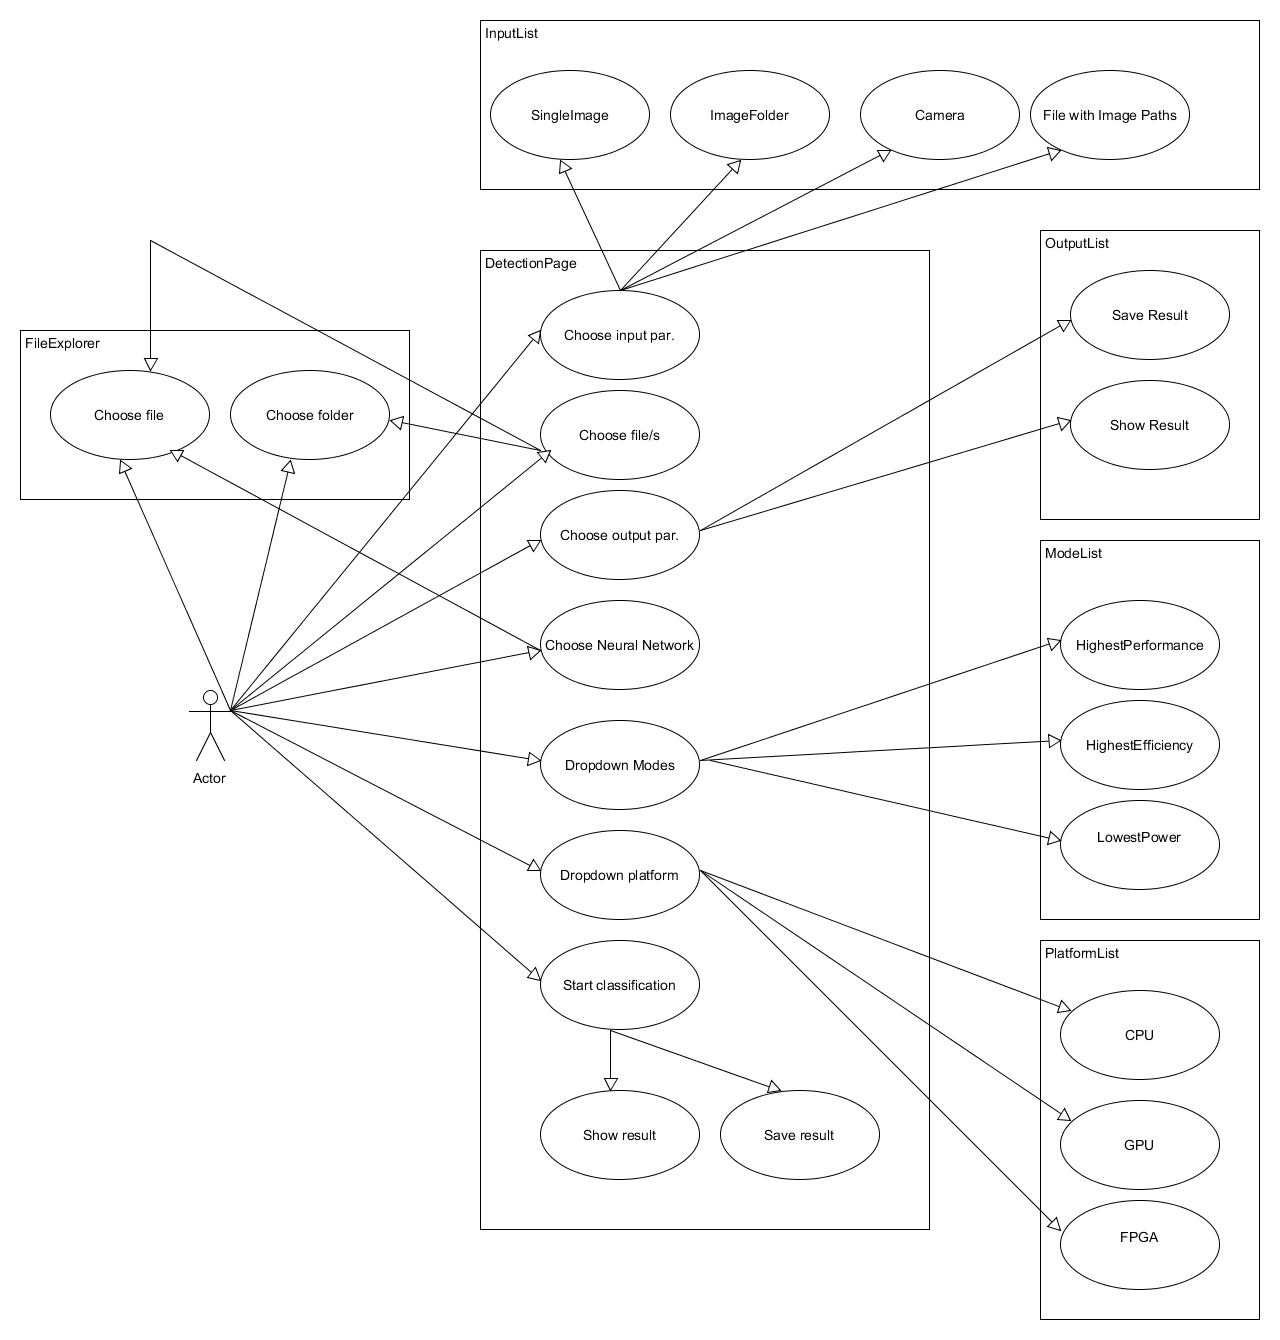
\includegraphics[width=\textwidth]{ClassificationUsecase}
\caption{Usecase of the image classification page}
\end{figure}
\subsubsection{Training page}
\begin{figure}[htb!]
\centering
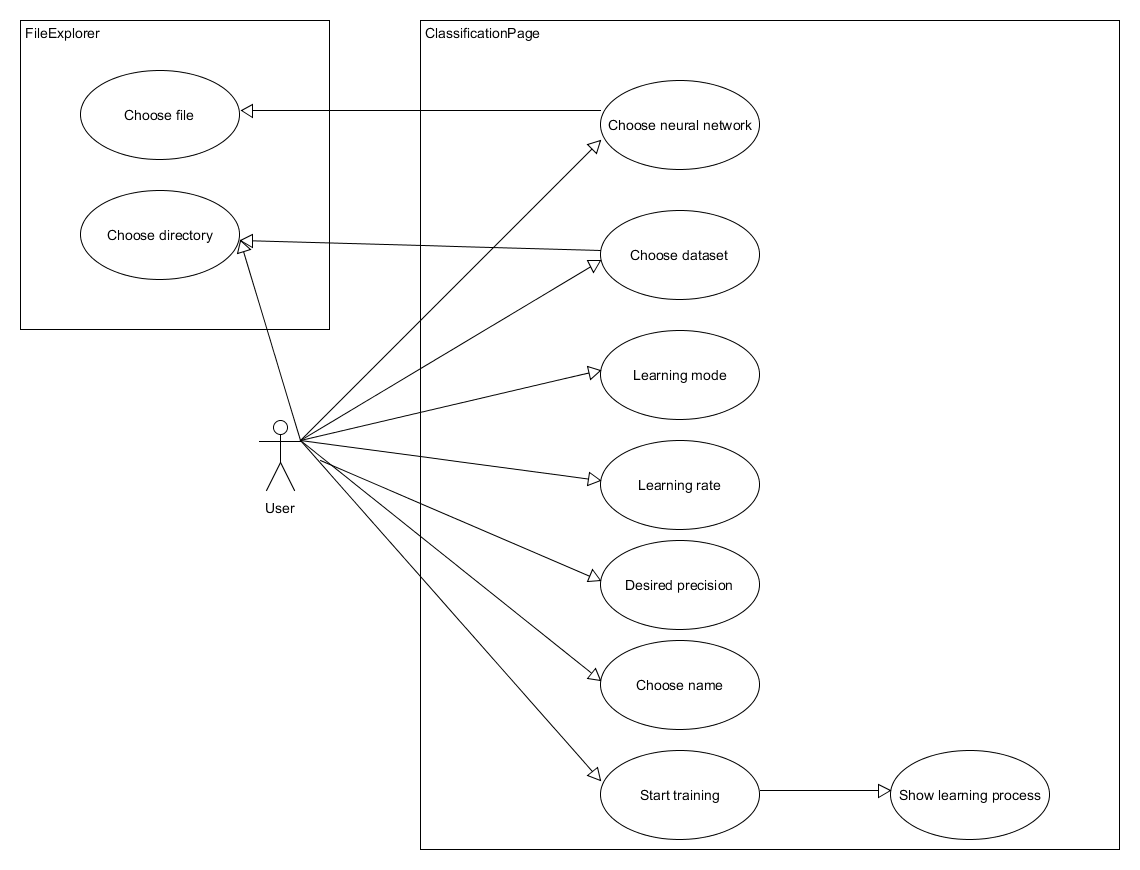
\includegraphics[width=\textwidth]{TrainUsecase}
\caption{Usecase of the trainingspage}
\end{figure}
\clearpage

\subsection{GUI}
\begin{figure}[htb!]\centering
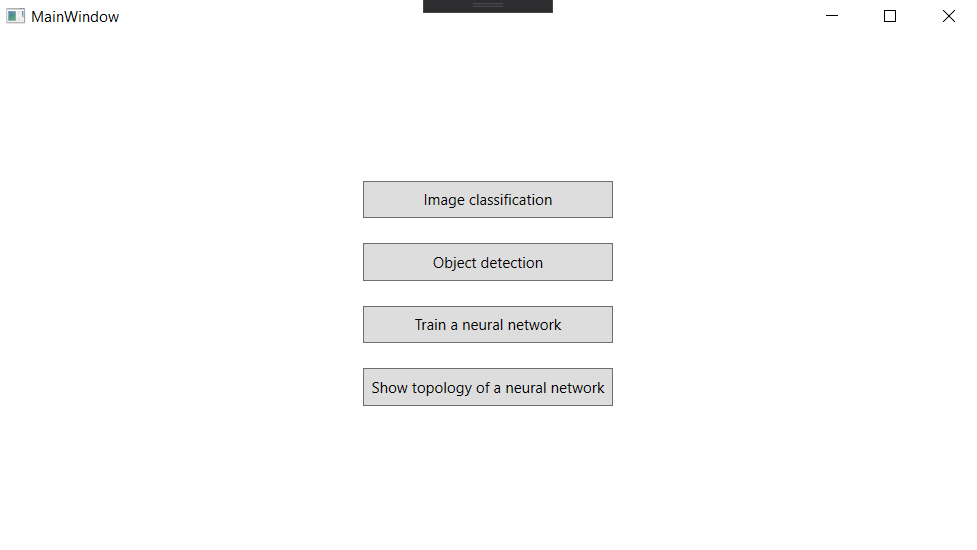
\includegraphics[width=\textwidth]{MainPageGUI}
\caption{Main page of our software}
\end{figure}
\begin{figure}[htb!]\centering
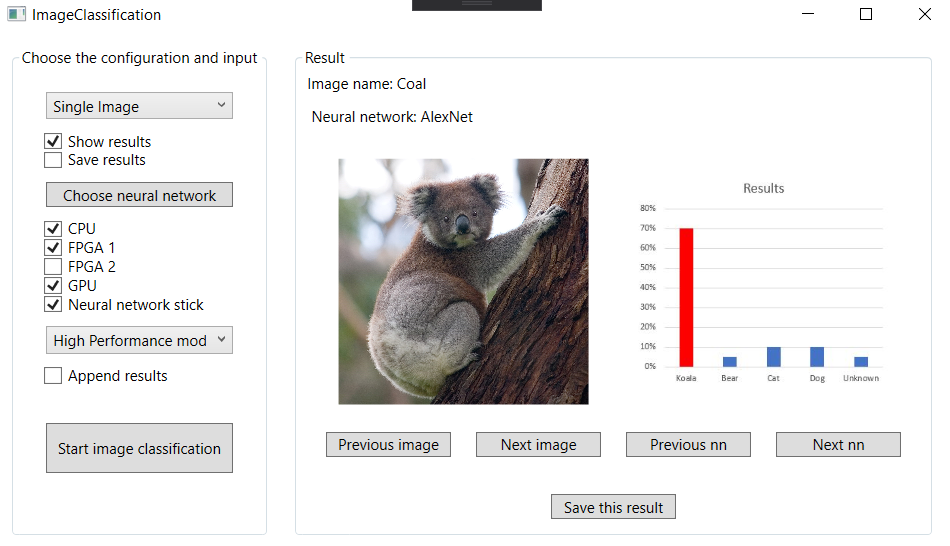
\includegraphics[width=\textwidth]{ImageClassificationGUI}
\caption{Image classification page of our software}
\end{figure}
\begin{figure}[htb!]\centering
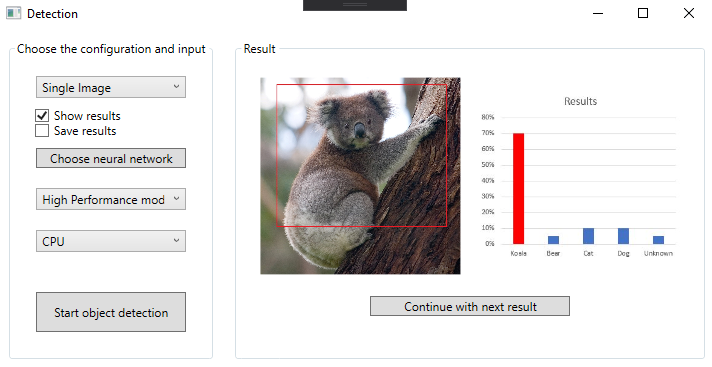
\includegraphics[width=\textwidth]{DetectionGUI}
\caption{Object detection page of our software}
\end{figure}
\begin{figure}[htb!]\centering
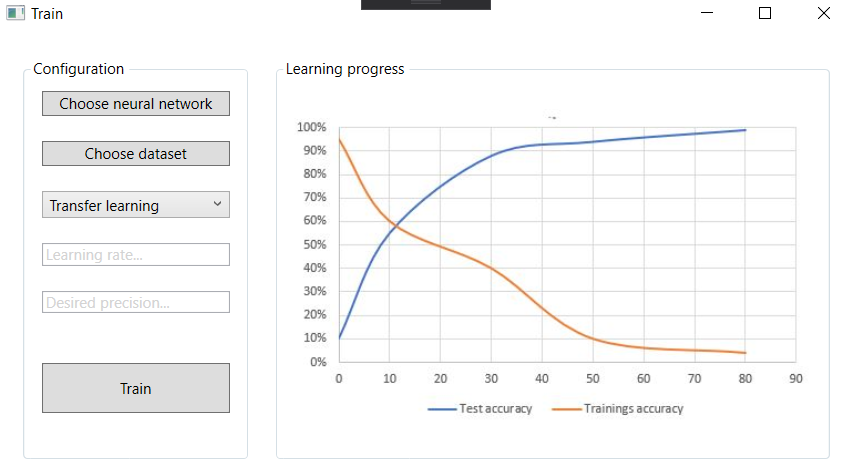
\includegraphics[width=\textwidth]{TrainGUI}
\caption{Training page of our software}
\end{figure}
\begin{figure}[htb!]
\centering
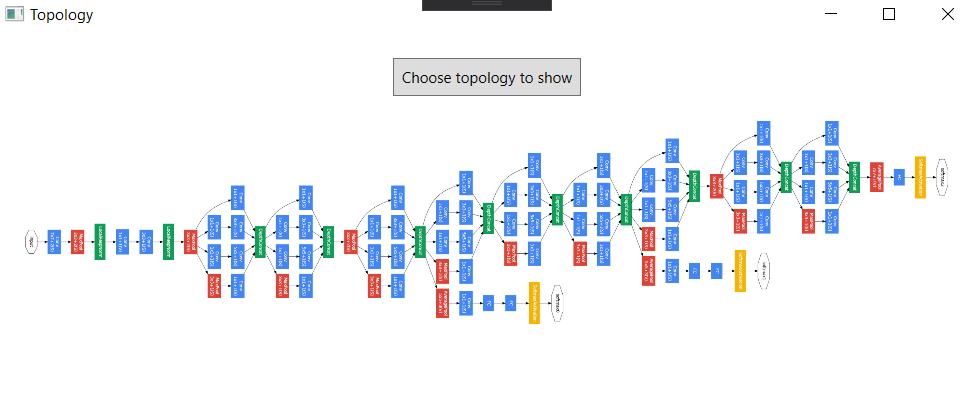
\includegraphics[width=\textwidth]{TopoGUI}
\caption{Page which shows the topology of a selected NN of our software}
\end{figure}
\clearpage

\section{Stage responsibilities}
\begin{tabular}{p{4cm}p{8cm}}
\textbf{Requirements:} & Paul Stangel\\
\textbf{Design:} & Johannes Häring\\
\textbf{Implementation:} & Manuel Drehwald\\
\textbf{Quality insurance:}& Stefani Guneshka\\
\textbf{Deployment:} & Dimitar Dimitrov
\end{tabular}
\clearpage

\printnoidxglossaries
\end{document}

